\chapter{The Large Hadron Collider and the CMS experiment}
\label{sec:chap_2}

The work presented in this thesis is based on data collected by the Compact Muon Solenoid (CMS) experiment, 
one of the four main experiments together studying the collisions 
provided by the Large Hadron Collider (LHC). A detailed description of the LHC and of the CMS 
experiment can be found in \cite{Evans:2006tq} and \cite{Chatrchyan:2008aa} respectively.
In this chapter we summarize the main features that are relevant for this work.

\section{The Large Hadron Collider}

The LHC and its experiments were built to explore the high-energy frontier of particle physics and to address fundamental questions of this field, such as the existence of a Higgs boson \cite{Englert:1964et,Higgs:1964ia,Higgs:1964pj,Guralnik:1964eu,Higgs:1966ev,Kibble:1967sv}, of extended symmetries \cite{Martin:1997ns}, extra dimensions \cite{Antoniadis:1999bq}, or new elementary particles \cite{Beltran:2010ww,Randall:1999vf}. All these phenomena don't have a well-defined energy range predicted by theory but they are expected to manifest at the TeV scale in case they exist in nature. A proton-proton collider was considered to be the most suitable machine for such a task, allowing higher energies with current technologies and probing a wide energy range.% at the same time exploiting the compositeness of the colliding particles.

The LHC is housed in the 27 km long underground tunnel where the Large Electron Positron collider (LEP) has been operating until its decommissioning in 2000. The tunnel is located under both French and Swiss territory, in proximity of the CERN research facility. 
Protons produced from hydrogen ionization are accelerated by a chain of older accelerators, some of them dating back to the late 1950's, before entering the LHC. %Before being accelerated in the LHC, protons are produced from hydrogen ionization and then accelerated through a chain of smaller machines, some of them dating back to the late 1950's. 
A schematic view of the CERN accelerators and their connection is shown in Figure \ref{fig:cern_accelerators}. From the last element of this chain, the Super Proton Syncrotron (SPS), protons are injected in the LHC with an energy of 450 GeV in two separate beam pipes, one containing protons running clockwise, the other with protons running in the opposite direction. Protons are bent in their trajectory by 1\,232 superconducting dipole magnets and focused by  superconducting quadrupole magnets, while 16 superconducting radio-frequency (RF) stations 
%provide the thrust to 
accelerate the two beams up to 7 TeV in steps of 0.5 MeV each turn. In order to maintain their superconducting properties the magnet coils and the cavities are cooled to a temperature of 1.9 K by a complex cryogenic system using superfluid helium as refrigerator. RF cavities can be used for accelerating the protons only if the beam is not continuous but structured in bunches. By design the LHC is built to contain 2808 bunches of $10^{11}$ protons each, giving a bunch time separation of 25 ns.
%Due to space constraints both the beam pipes are encased in the same dipole and the proper magnetic field direction is achieved with a particular magnet design.  

\begin{figure}
\begin{center}
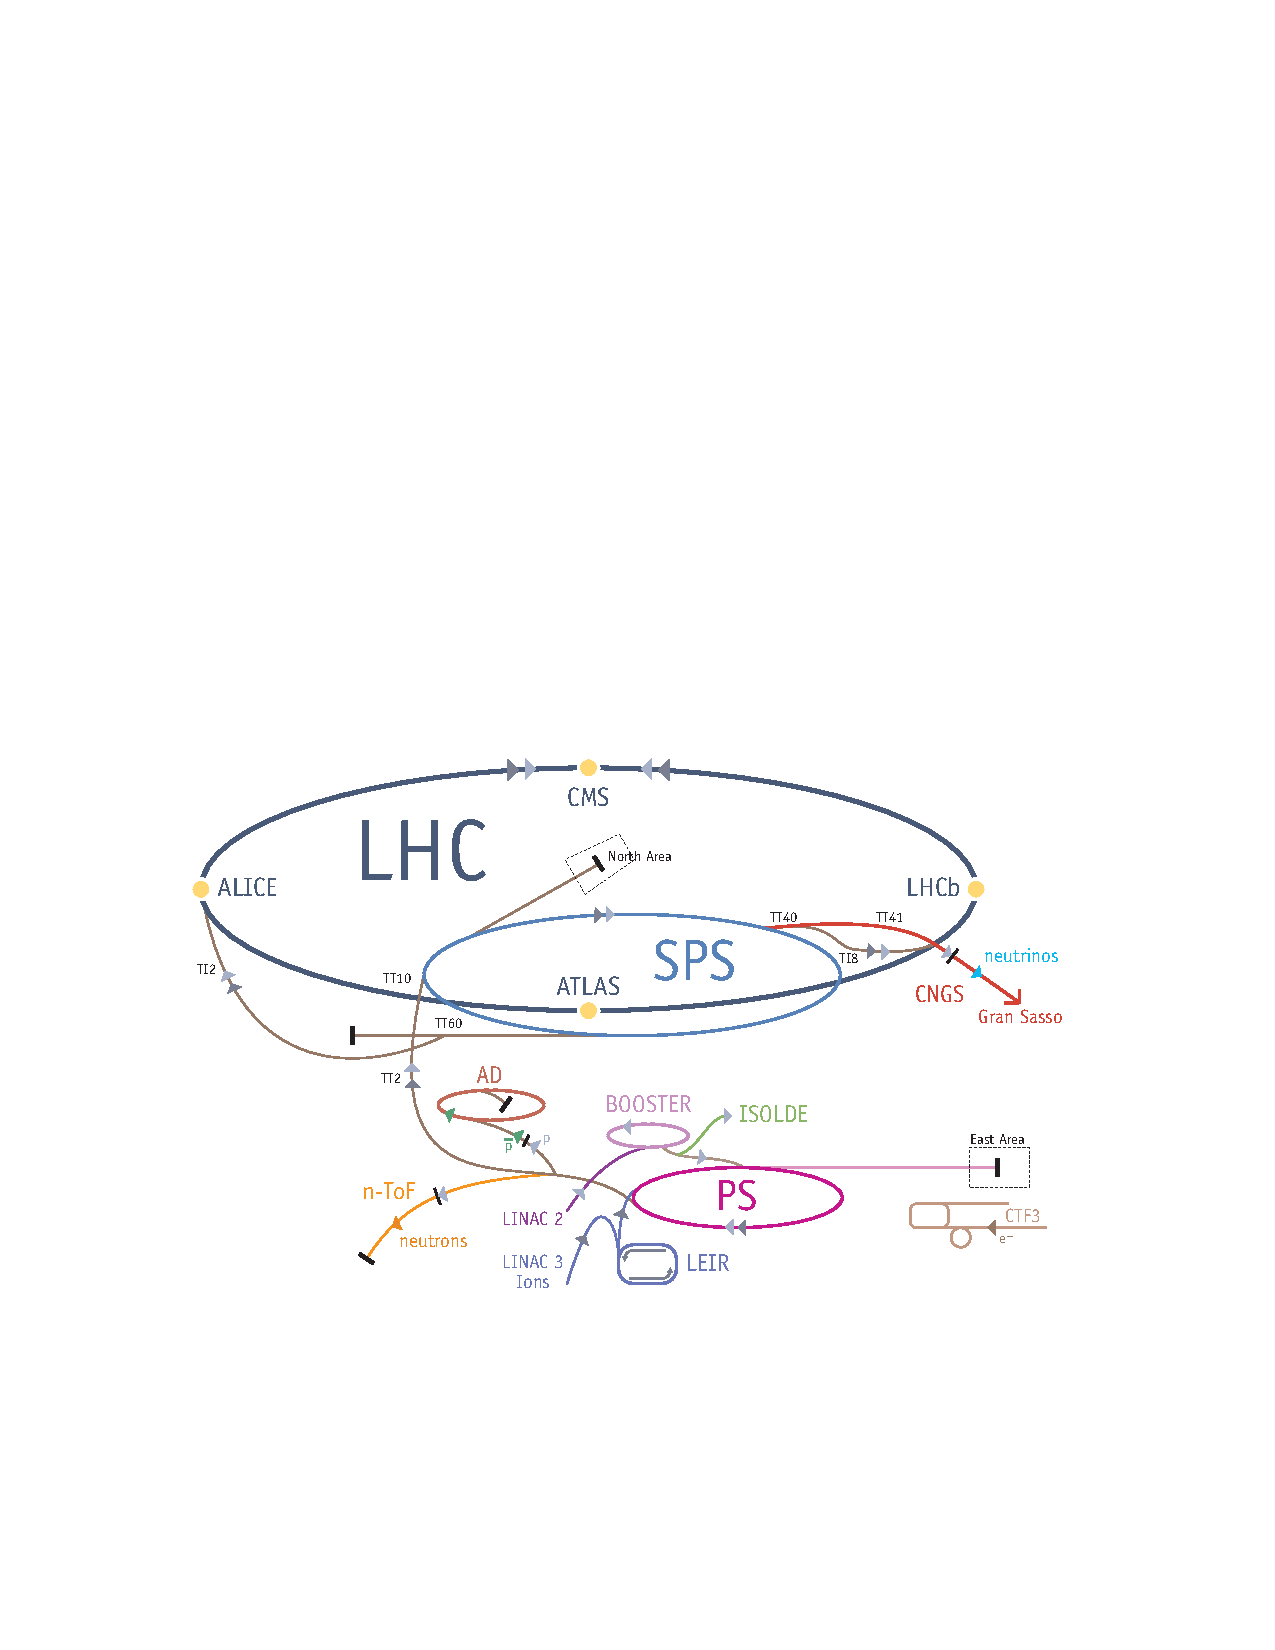
\includegraphics[angle=-0,width=0.8\textwidth]{2_LHC_and_CMS/pics/LHC.pdf}
\caption{Schematic view of the CERN accelerators and their connection
\label{fig:cern_accelerators}
}
\end{center}
\end{figure}

The LHC started its operation on 10 September 2008 and after only 9 days of operation a severe \emph{quenching} of about 100 dipole magnets, causing the release of around two tonnes of helium, forced the machine to stop and to address some design failures. The main cause of the accident was found to be in some of the electrical connections between magnets. In 2009 the machine became operational again, with a reduced beam energy, in odrer to reduce the current flowing in the dipole magnets. The year 2010, after a careful ramp-up of the beam energies, saw the start of the LHC research program with collisions at a center-of-mass energy of $\sqrt{s} = 7$ TeV, half of the design value. During 2010 and 2011 the machine commissioning continued along with the data taking. During this time the instantaneous luminosity increased continuously. The beam energy was raised to 4 TeV, corresponding to $\sqrt{s} = 8$ TeV center-of-mass energy, in 2012. The LHC design specifications and the performance achieved so far are summarized in table \ref{tab:lhc_figures}. The LHC is scheduled to start a new data-taking run in 2015 at a center-of-mass energy of $\sqrt{s} = 13$ TeV.

\begin{table}[h!]
   \centering
  \caption{Relevant LHC machine parameters. The design values are compared to the ones reached during the 2013 operations.}
\begin{tabular}{c|ccccc}
\hline
Parameter & Design value&  Best value achieved \\ 
\hline
Beam energy   & 7 TeV & 4 TeV \\ 
Number of protons per bunch & 1.15$\times$10$^{11}$ & 1.5$\times$10$^{11}$ \\
Number of bunches & 2808 & 1368 \\
Crossing angle & 300~\si{\micro\metre} & 290~\si{\micro\metre} \\
Beam size & 17~\si{\micro\metre} & 20~\si{\micro\metre} \\
Emittance & 3.75 ~\si{\micro\metre} & 2.4~\si{\micro\metre}  \\
Peak luminosity & $10^{34}$~cm$^{-2}$s$^{-1}$ & 7.5$\times$10$^{33}$~cm$^{-2}$s$^{-1}$ \\
\hline
\end{tabular}
  \label{tab:lhc_figures}                
\end{table}


The instantaneous luminosity,$\operatorname{\mathcal{L}}(t)$, is the number of particles per unit area per unit time available for collisions. For any given physics process the average number of events is given by:

\begin{equation} 
	N_{ev} = \sigma\int\operatorname{\mathcal{L}}(t)\mathrm{d}t,
	\label{eq:n_events}
\end{equation} 

where $\sigma$ represents the cross-section for the studied process. While the cross section depends on the process, the instantaneous luminosity is entirely derived from accelerator parameters:

\begin{equation} 
	\operatorname{{\cal L}}(t) = \frac{N_p^2 n_b f_{rev} \gamma }{4 \pi \epsilon_{n} \beta^*} F
	\label{eq:lumi}
\end{equation} 

where $N_p$ and $n_b$ are the number of protons per bunch and the total number of bunches respectively, $f_{rev}$ is the rotation frequency, $\epsilon_{n}$ and $\beta^*$ describe the beam focusing at the interaction point, $\gamma = E_p / m_p$ is the Lorentz factor of the protons in the beam and $F$ accounts for the crossing angle between the two beams. Although the number of bunches has always been less than half the design value during all the running period, the peak instantaneous luminosity has been only 30\% lower than the design one. This result was achieved by increasing the number of protons in each bunch and increasing the focusing of the beams. The price to pay for the high luminosity, in particular in the second half of 2011 and in 2012, was an increase of the average number of proton collisions per bunch crossing, the so-called \emph{pileup}. This effect is displayed in figure \ref{fig:lhc_pileup} where the peak number of simultaneous interactions per bunch crossing recorded by the CMS detector is shown as a function of time.

\begin{figure}
\begin{center}
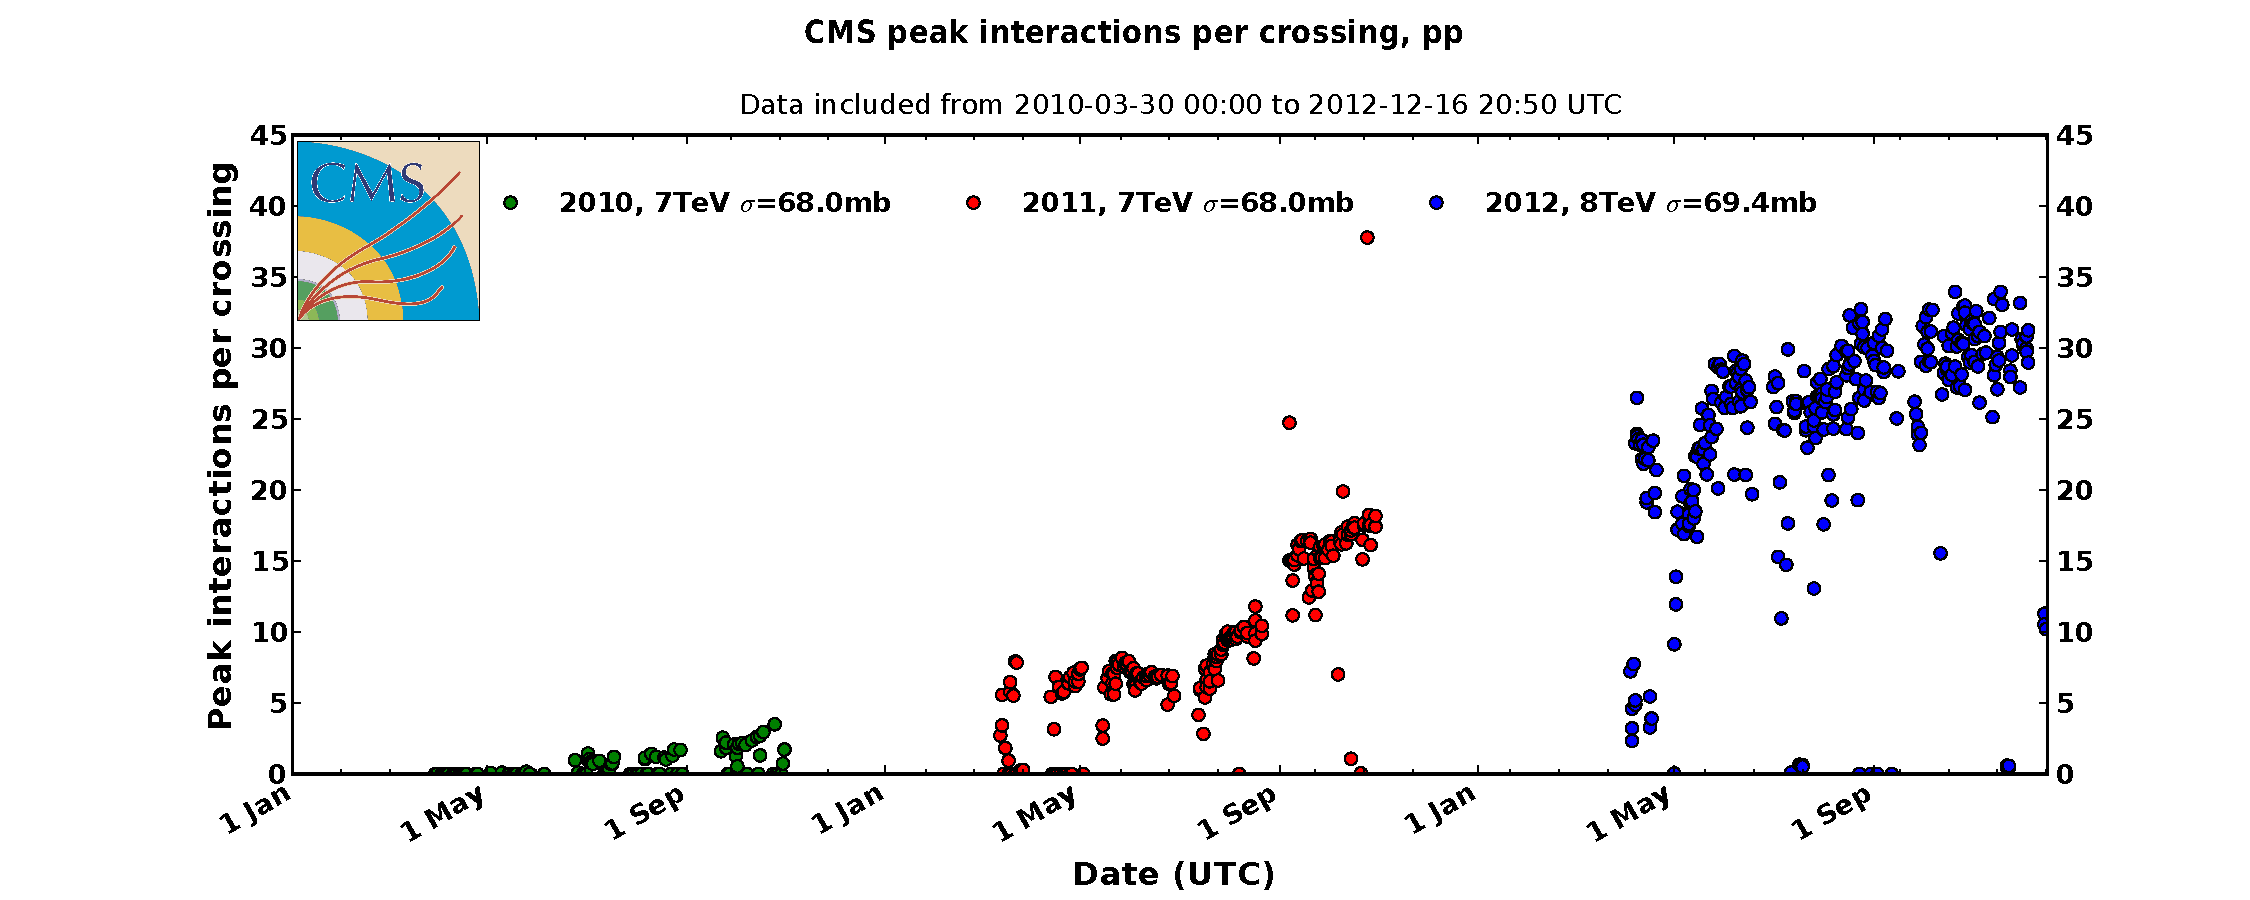
\includegraphics[angle=-0,width=\textwidth]{2_LHC_and_CMS/pics/peak_pu_pp.pdf}
\caption{Peak Interactions per crossing versus time for p-p collisions (includes special runs), each point represents a fill. This is shown separately for the 2010 (green), the 2011 (red) and the 2012 (blue) data-taking periods.
\label{fig:lhc_pileup}
}
\end{center}
\end{figure}

The integrated luminosity is usually quoted as \L. During its operations the LHC delivered 44.2~pb\Inv in 2010, 6.1~fb\Inv in 2011 and 23.3~fb\Inv at 8~TeV in 2012. The progress of the accelerator in terms of integrated luminosity is shown in Figure \ref{fig:int_lumi}.

\begin{figure}
\begin{center}
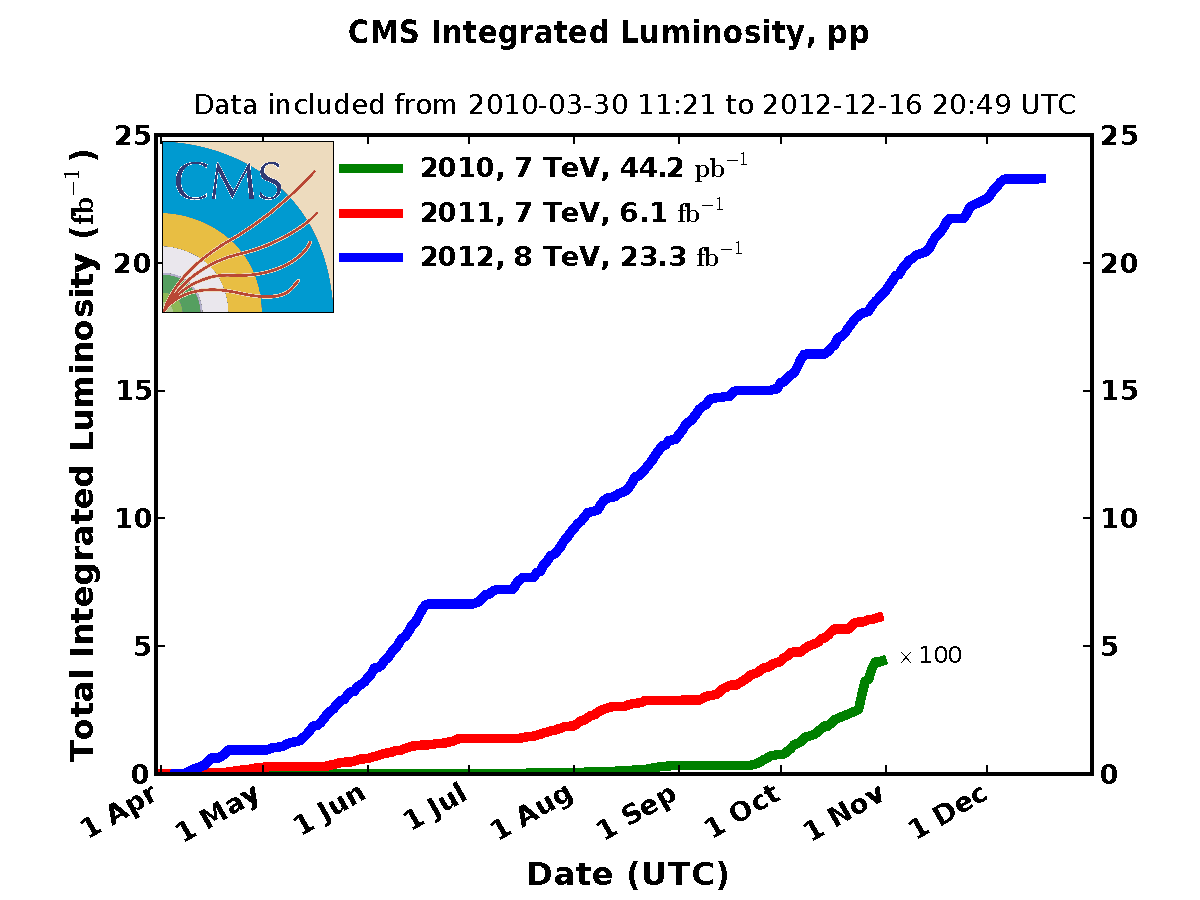
\includegraphics[angle=-0,width=0.8\textwidth]{2_LHC_and_CMS/pics/int_lumi.pdf}
\caption{Integrated luminosity delivered to CMS during stable beams and for p-p collisions as a function of time, shown separately for the 2010 (green), the 2011 (red) and the 2012 (blue) data-taking periods.
\label{fig:int_lumi}
}
\end{center}
\end{figure}


\section{The CMS detector}

The CMS detector is located in the LHC tunnel at point 5, near the French town of Cessy, between the Jura mountains and the Geneva lake.
 
The CMS experiment, together with ATLAS, constitutes one of the two multi-purpose detectors operating at the LHC. Its primary task is to probe particle physics at the TeV scale searching for new phenomena as well as for the Higgs boson, the only missing piece to the SM puzzle. The experiment is also well suited to perform precision measurements of standard model processes and flavor physics studies. A heavy-ion program is carried on as well to probe QCD at very high energies and matter densities, trying to reproduce an environment similar to the conditions of the universe few instants after the Big Bang.

To carry out such ambitious research program the detector was designed to meet some baseline requirements:
\begin{itemize}
\item Good muon identification and momentum resolution over a wide range of momenta and angles with di-muon mass resolution of ~1\% at 100~GeV.
\item Ability to identify the muon charge without any ambiguity for muons momenta below 1~TeV
\item Good charged-particle momentum resolution, high tracking efficiency and resolution. These characteristics are especially important for objects like \b-jets and tau leptons, where isolated charged hadrons and displaced vertices play a fundamental role. A high tracking resolution also plays a key role in assigning the tracks to the production vertex, mitigating the effect of pileup.
\item Good electromagnetic energy resolution, with a di-photon invariant mass resolution of \~1\% at 100~GeV and wide geometric coverage with efficient photon and lepton isolation in high pileup conditions.
\item Hermetic hadronic calorimeter with fine transverse segmentation for good jet mass and missing transverse energy ($E_T^{miss}$) resolution. 
\end{itemize}

The total proton-proton cross section at 14~TeV is expected to be roughly 100~mb, leading to an average of 20 pileup interactions with LHC design values. This value has been exceeded during the 2012 data taking period already. The number of \emph{pileup} events together with the short 25~ns bunch spacing pose stringent requirements on the resolution, granularity and latency of the different subdetectors. The ability to resolve overlapping vertices and assign their respective track is of primary importance. A fast trigger system is also required to reduce the event rate from the design collision rate of 40~MHz to 300Hz, the maximum rate foreseen for storing events permanently.

In order to meet all these requirements CMS has been built with a 4~T NbTi superconducting solenoid magnet with an inner diameter of 6 m. Inside the magnet a large silicon tracker, the largest of its kind, is housed to track charged particles with the required resolution. Around the tracker, but still within the solenoid field, a lead-tungstanate electromagnetic calorimeter (ECAL) and a brass-scintillating sampling hadron calorimeter (HCAL) are installed. Inside the 1.5~m thick iron return yoke of the magnet four muon stations are installed. They consist of several layers of drift tubes or cathode strip chambers complemented by resistive plate chambers. A schematic view of a transverse slice of the CMS detector is presented in Figure \ref{fig:cmsdet}

\begin{figure}
\begin{center}
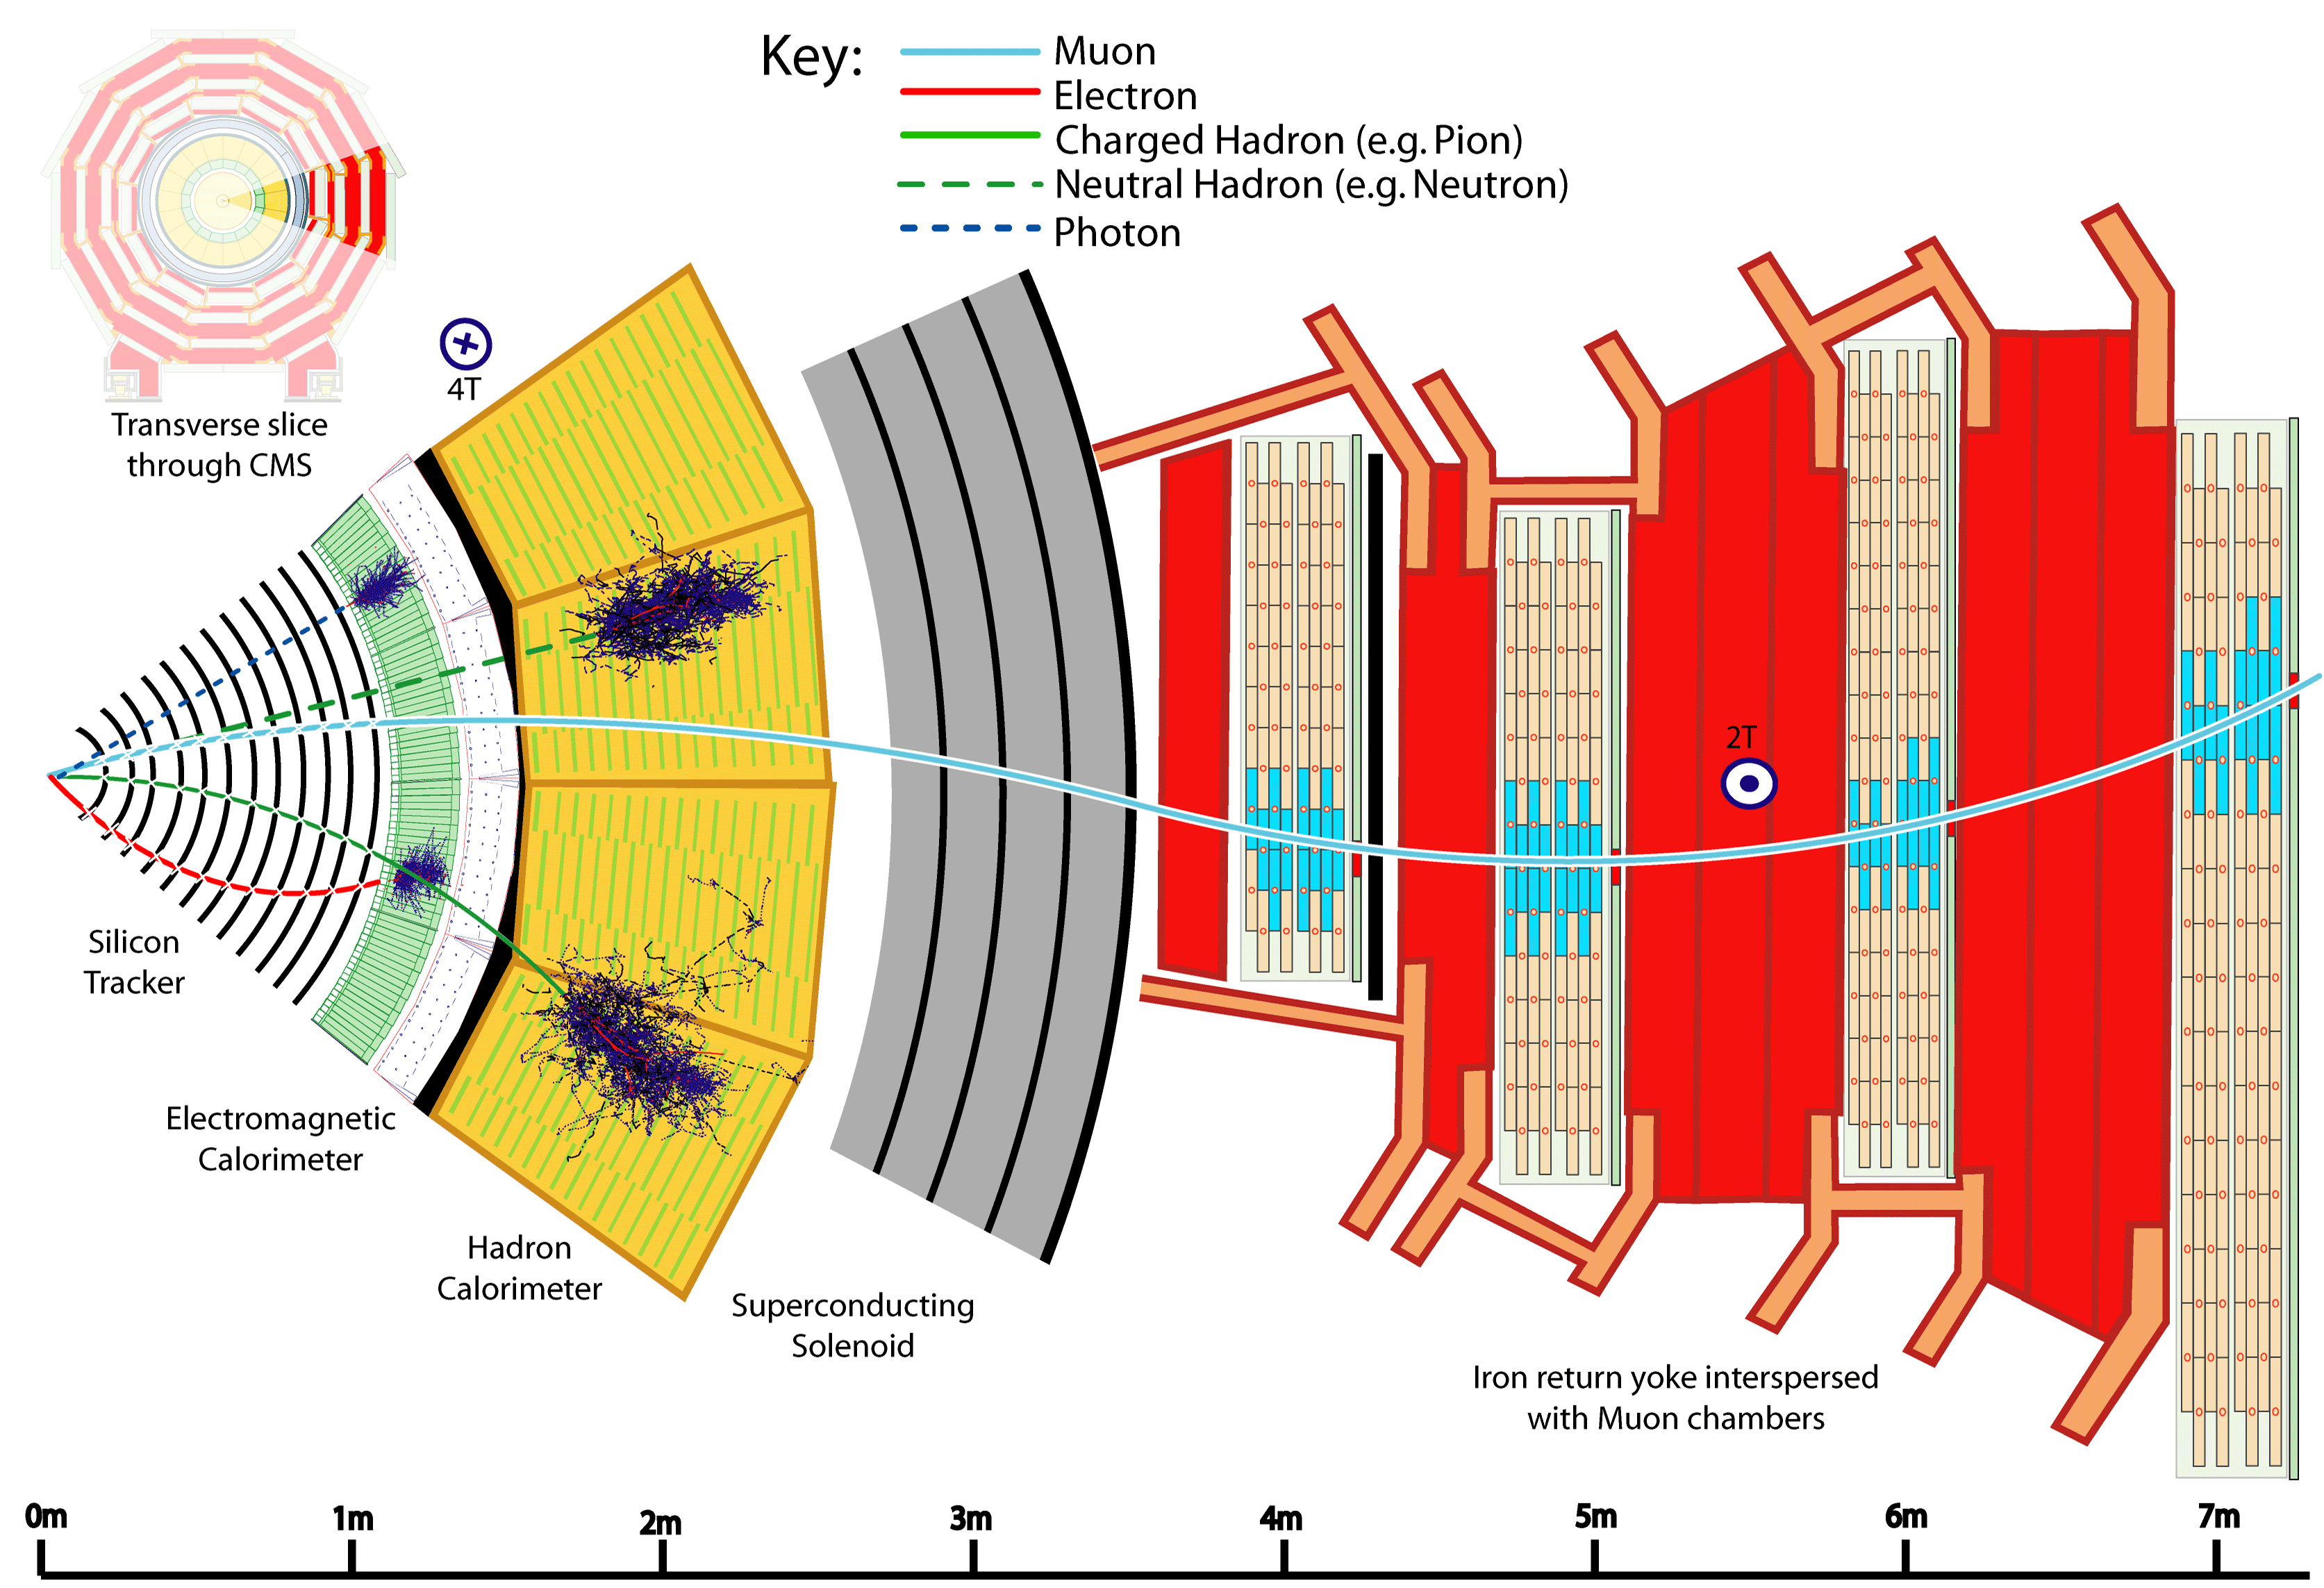
\includegraphics[angle=-0,width=0.8\textwidth]{2_LHC_and_CMS/pics/CMS_Slice_HD.png}
\caption{Transverse slice of the CMS barrel section, showing the trajectory of different types of particles crossing the detector and the typical signal they leave in each subdetector.
\label{fig:cmsdet}
}
\end{center}
\end{figure}


\paragraph{The coordinate system}
chosen by CMS has the $y$ axis pointing vertically upward and the $x$ axis pointing horizontally towards the center of LHC. The $z$ axis is oriented along the beam line, pointing in the direction of the beam that runs anti-clockwise and points towards the Jura. A set of polar coordinates is used to describe the $xy$ plane in the form of radius $r$ and angle $\phi$, while the angle $\theta$ is measured with respect to the positive $z$ axis direction. Usually the polar angle $\theta$ is replaced by the \emph{pseudorapidity}, defined as $\eta=-\ln \tan(\theta/2)$, which is Lorentz invariant for boosts along the $z$ axis and therefore comes very handy when describing processes for which the longitudinal boost is unknown. The three-dimensional angular distance is also replaced by its Lorentz-invariant $\D R=\sqrt{\D\phi^2+\D\eta^2}$, where $\D\eta$ and $\D\phi$ are the $\eta$ and $\phi$ coordinate differences of two points.

\subsection{Inner Tracker}
\label{sec:inner_tracker}

The inner tracker provides the essential spatial information needed to reconstruct charged tracks as well as primary and secondary vertices. A schematic view of the inner tracker is shown in figure \ref{fig:tracker}. To cope with the very high track density and to provide the best spatial resolution, the innermost part of the tracker is based on silicon pixel technology. The pixel detector, displayed in figure \ref{fig:pixel}, is composed of three cylindrical layers at distances of 4.4, 7.3 and 10.2 cm with respect to the beam axis complemented by two disks  in the forward and backward regions. The total active area of the pixel detector is about of 1 m\sq.  It provides bi-dimensional measurements within its angular acceptance: $|\eta| \leq 2.5$. The pixel cell size is 100 $\times$ 150 \u m\sq. 
The solenoidal magnetic field drift spreads the charge deposited in the sensors on several neighboring pixels allowing for a better hit resolution.
To enhance this effect in the forward wheels the sensors are placed in a turbine-like geometry. The combination of analogue read-out and usage of the charge sharing information allows to achieve a spatial resolution of 9-33 \u m per hit \cite{trackingpaper}. 

The pixel detector can be extracted from the rest of the tracker to allow easy access for maintenance without interfering with the rest of the detector. This feature is particularly important due to the high radiation dose that the first layers of the pixel detector sustain, requiring additional maintenance.

\begin{figure}
\begin{center}
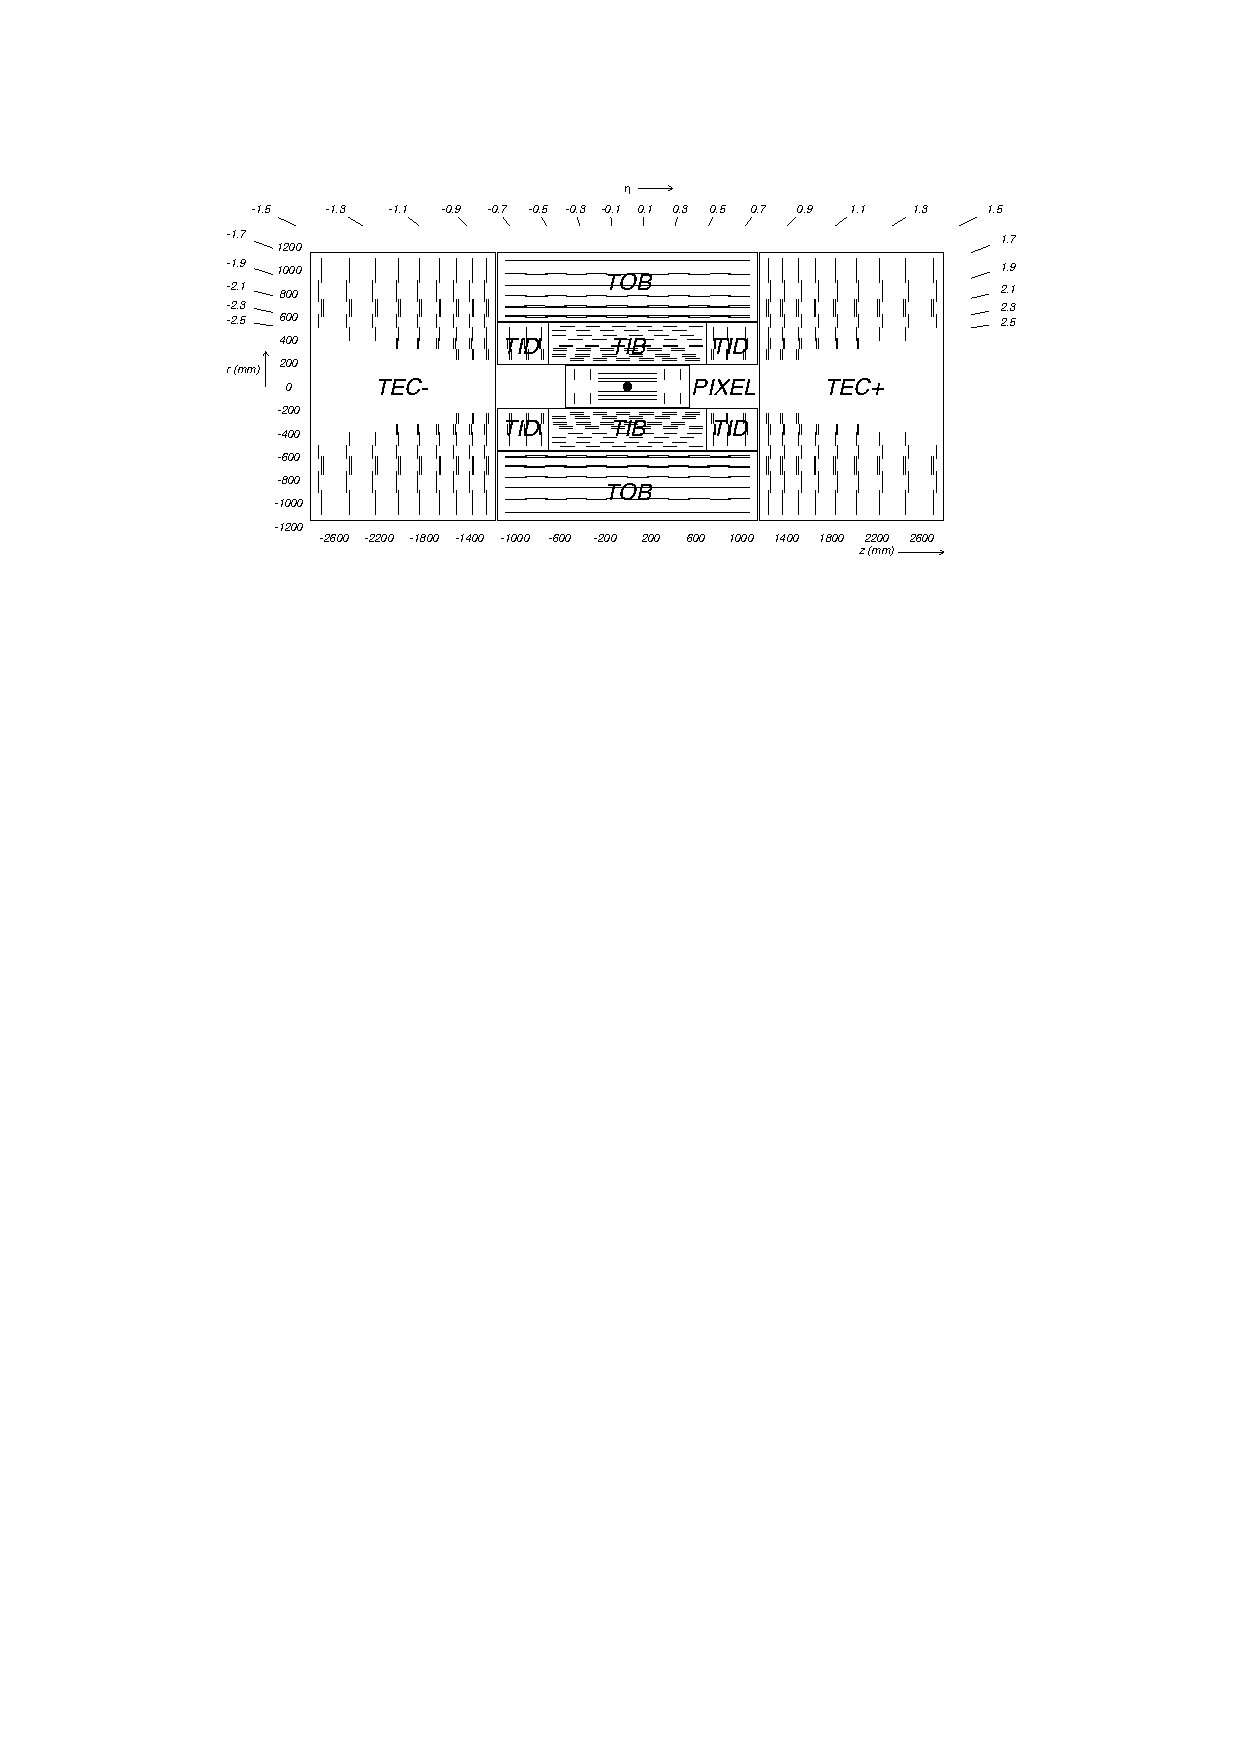
\includegraphics[angle=-0,width=0.8\textwidth]{2_LHC_and_CMS/pics/trkxsec.pdf}
\caption{Longitunal cross section of the CMS tracker, with pseudo rapidity coverage of the different detector elements. 
\label{fig:tracker}
}
\end{center}
\end{figure}

\begin{figure}
\begin{center}
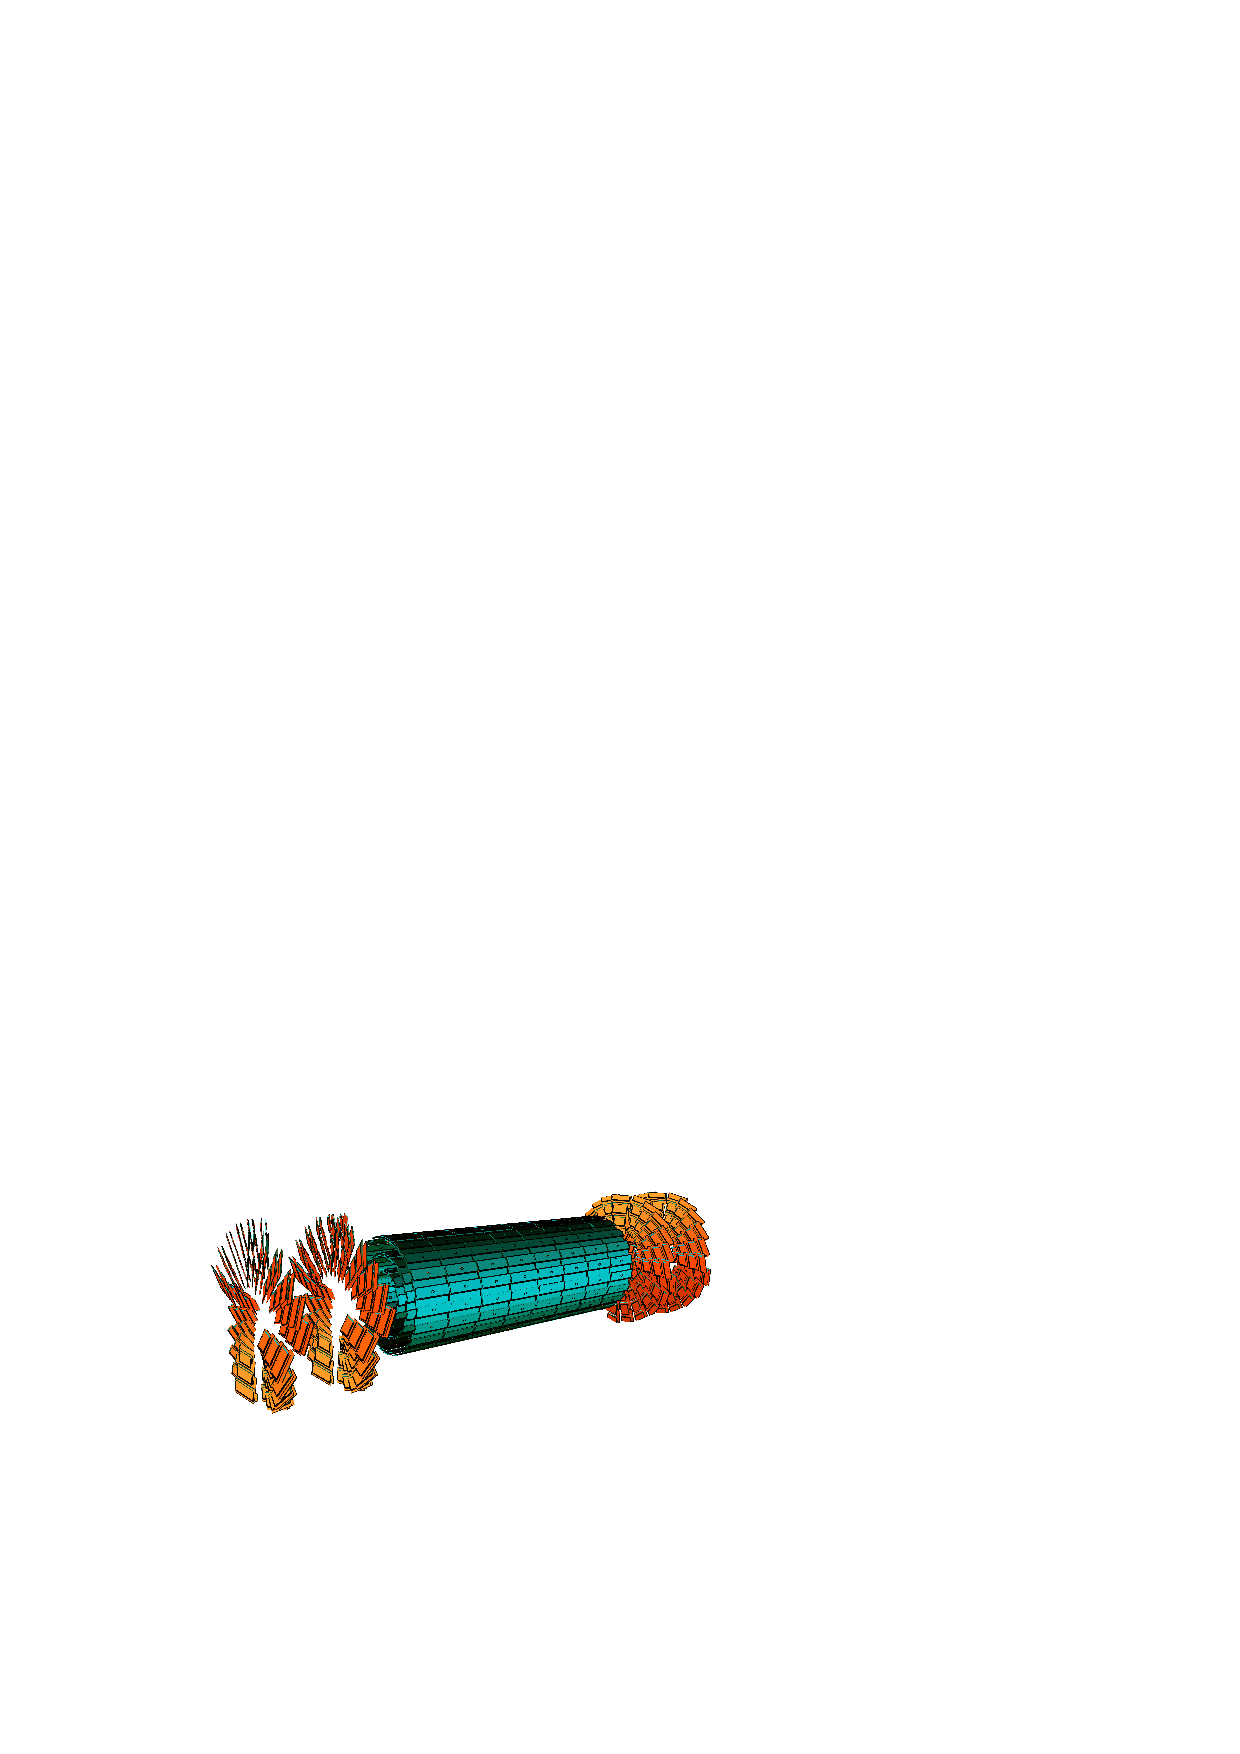
\includegraphics[angle=-0,width=0.8\textwidth]{2_LHC_and_CMS/pics/pixelfull.pdf}
\caption{Three dimensional sketch of the CMS pixel detector, barrel modules in blue and endcap wheels in orange.
\label{fig:pixel}
}
\end{center}
\end{figure}

The outer layers of the tracker are made of silicon strip detectors and further divided into four sections: tracker inner and outer barrel (TIB and TOB), tracker inner disks (TID) and tracker endcaps (TEC), as illustrated in figure \ref{fig:tracker}. TIB and TID are located at distances between 20 and 55 cm from the beam line. They consist of four barrel layers and three disks at each end. The sensors are made of 320 \u m thick silicon with a strip pitch that varies from 80 \u m in the innermost barrel layer to 140 \u m in the outermost disks. The combination of TIB and TID delivers up to four transverse measurements. The TIB-TID sections are surrounded by the TOB, which fills the remaining space up to a radius of 116 cm from the beam line. It consists of six barrel layers of 500 \u m thick sensors with a strip pitch of 183 \u m for the first four layers and 122 \u m for the remaining two. The TEC is located in the end-cap region and extends from a radius of 20 cm to 113.5 cm, and $|z| > 118$ cm. It consists of nine disks. Each disk is composed by up to seven concentric rings of strip sensors. The thickness and the strip pitch of the sensor vary depending on the distance from the beam line. 

Intrinsically strip sensors only provide one dimensional spatial information ($\phi$). In order to measure a second coordinate ($r$ for disks, $z$ for barrel), an additional set of sensors is mounted back-to-back with a stereo angle of 100 mrad on the first two layers of TIB, TID and TOB and on layers 1, 2 and 5 of TEC. The strip tracker geometry is designed such that particles originating from the nominal interaction point typically cross nine or more layers of sensors, with at least four of them providing two-dimensional information.

%temperatura?

\subsection{Electromagnetic Calorimeter}

The CMS electromagnetic calorimeter (ECAL) surrounds the inner tracker. It is divided into ECAL Barrel (EB), covering the pseudo rapidity range $|\eta| < 1.479$, and ECAL Endcaps (EE), which covers the range $1.479 < |\eta| < 3$. 
ECAL consist of 68\,524 scintillating lead tungstanate (PbWO$_4$) crystals, the light of which is read out by photomultipliers. 

The choice of lead tungstanate was driven by its high density yielding a short radiation length (0.89 cm) and small Moliere radius (2.2 cm), together with being radiation hard and yielding fast signals, with 80\% of the light yield emitted within 25~ns. To keep the calorimeter as hermetic as possible, the crystals have truncated pyramidal shape. One of the longitudinal faces is left unpolished, to moderate the non uniform light collection across the crystal length that this peculiar shape causes. Each crystal covers about $0.0174 \times 0.0174$ in the $\eta-\phi$ plane and is oriented such that its front face points towards the nominal interaction point (with a slight misalignment to mitigate the effect of the crystal surface on photon detection). The crystals are read-out by a pair of avalanche photodiodes (APD) in the barrel and by vacuum phototriodes in the endcap. Both the devices can operate in high magnetic fields with little or no efficiency degradation and exhibit a good radiation hardness.

A pre-shower detector is installed in front of the ECAL endcap, its purpose being to discriminate between single photons and photons from \piz decays, and to enhance the angular resolution of both electrons and photons. The pre-shower detector consists of a double-layer lead-silicon calorimeter, with the lead initiating the shower and the silicon strip detector placed after each lead layer to measure the deposited energy and shower profile with high granularity.

\subsection{Hadronic Calorimeter}

The hadronic calorimeter (HCAL) serves two purposes: it measures the energy of charged and neutral hadrons from the p-p interaction while stopping them, thus allowing only muons to pass through and avoiding large quantities of energy being deposited inside the superconducting magnet. As most of the other subdetectors HCAL is divided in a barrel section (HB), covering the region $|\eta| < 1.3$, and an endcap section (HE), covering the region $1.3 < |\eta| < 3$. Both sections are located inside the superconducting solenoid. HCAL is a sampling calorimeter with brass passive plates, in which the hadronic shower begins and develops, interspaced with active plastic scintillator which measures the shower profile and the energy deposited. 

The scintillator is segmented both in $\eta$ and $\phi$ to provide the necessary granularity. Each scintillating tile is connected to the readout by a wavelength-shifting fiber that runs in a groove machined into the tile. The fiber guides the light emitted by the scintillator to a hybrid photodiode (HPD). The HPDs consist of a photocathode kept at high voltage. Electrons emitted by the photocathode are accelerated in the short distance (\~3 mm) that separates the cathode from a silicon pixelated anode which amplifies the signal. These devices were chosen due to their high dynamic range, their high gain ($O(2000)$) and their capability to work in a magnetic field.

The effective thickness of the calorimeter in terms of interaction length, $\lambda_I$, ranges in the barrel from a minimum of 5.82 $\lambda_I$ at $\eta=0$ to a maximum of 10.6 $\lambda_I$ at $|\eta| = 1.3$. The ECAL crystals add about 1.1 additional interaction lengths. The total thickness of the endcap calorimeters, including the ECAL crystals, amounts to about 10 $\lambda_I$.

Due to the limited stopping power of HB, especially in the central rapidity region, an additional hadronic calorimeter is placed outside of the solenoid magnet (hadron outer or HO). Its function is that of a \emph{tail catcher}. The HO consists of one scintillating station (two for the most central region) exploiting the solenoid itself ( and the first return yoke in case of the second station) as absorber. The HO extends the total thickness of the hadron calorimeter to a minimum of $11 \lambda_I$.

\subsection{Muon System}

Muon detection and triggering are of prime importance in CMS, as many new physics processes may manifest themselves via decay chains involving muons. 
Muon detection in the channel $\rm{H}\To ZZ^\ast$ was also of prime importance for the discovery of the Higgs boson. %Among those, the decay of a Higgs boson into $\Z\Z^*\To4\mu$ stands out as one of CMS's flagship analyses and one of those leading to the discovery of the Higgs boson announced on July 4$^{th}$, 2012 \cite{Chatrchyan:2013lba}. 
For this reason a redundant system of three different kinds of detectors is used to track muons in CMS. 

The muon system, whose scheme is shown in figure \ref{fig:mudet}, is housed in gaps between the return yoke of the solenoid magnet in the outermost region of the experiment. It consists of a Drift Tube (DT) tracking system in the barrel and multi-wire proportional chambers in the end-cap. In addition, a set of Resistive Plate Chambers (RPC) is located both in the barrel and in the endcap regions, providing a better time resolution  in the region of high particle activity, at the cost of coarser spatial resolution. 

\begin{figure}
\begin{center}
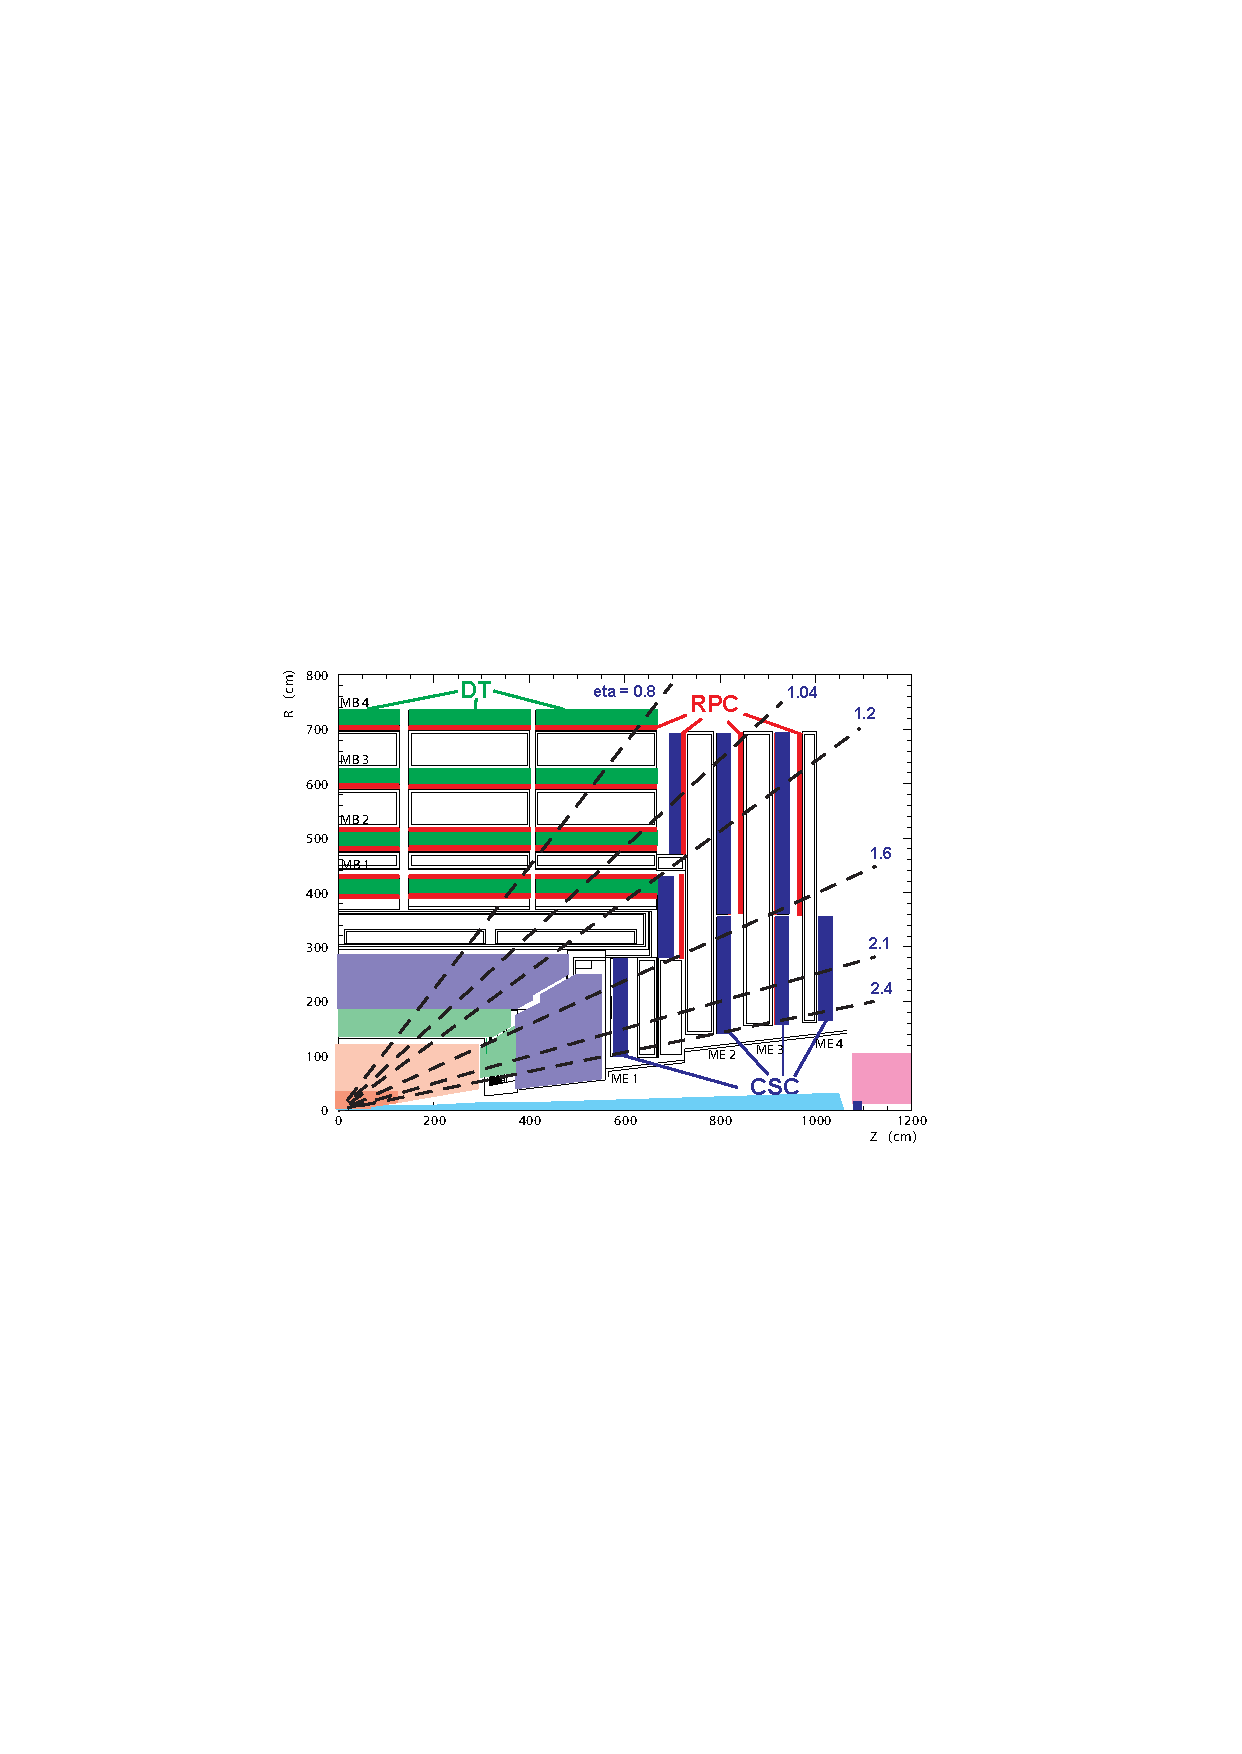
\includegraphics[angle=-0,width=0.8\textwidth]{2_LHC_and_CMS/pics/mudet.pdf}
\caption{Longitudinal cross-section of the CMS detector showing the location of the muon system.
\label{fig:mudet}
}
\end{center}
\end{figure}

\subsubsection*{Drift Tubes}

Drift tubes are employed to identify and track muons in the barrel region ($|\eta| < 1.2$), where the rate is below 1 Hz/cm\sq ~and the residual magnetic field less than 1 T, allowing for the usage of this technology. Four muon stations are located at increasing distance from the beam line. The first three stations are equipped with two \emph{super-layers} (SL) that provide a measurement of the $\phi$ coordinate and one SL that measures the $z$ one, as can be seen in figure \ref{fig:dt_module}, representing one DT module. In the last station the SL measuring the $z$ coordinate is missing. 

\begin{figure}
\begin{center}
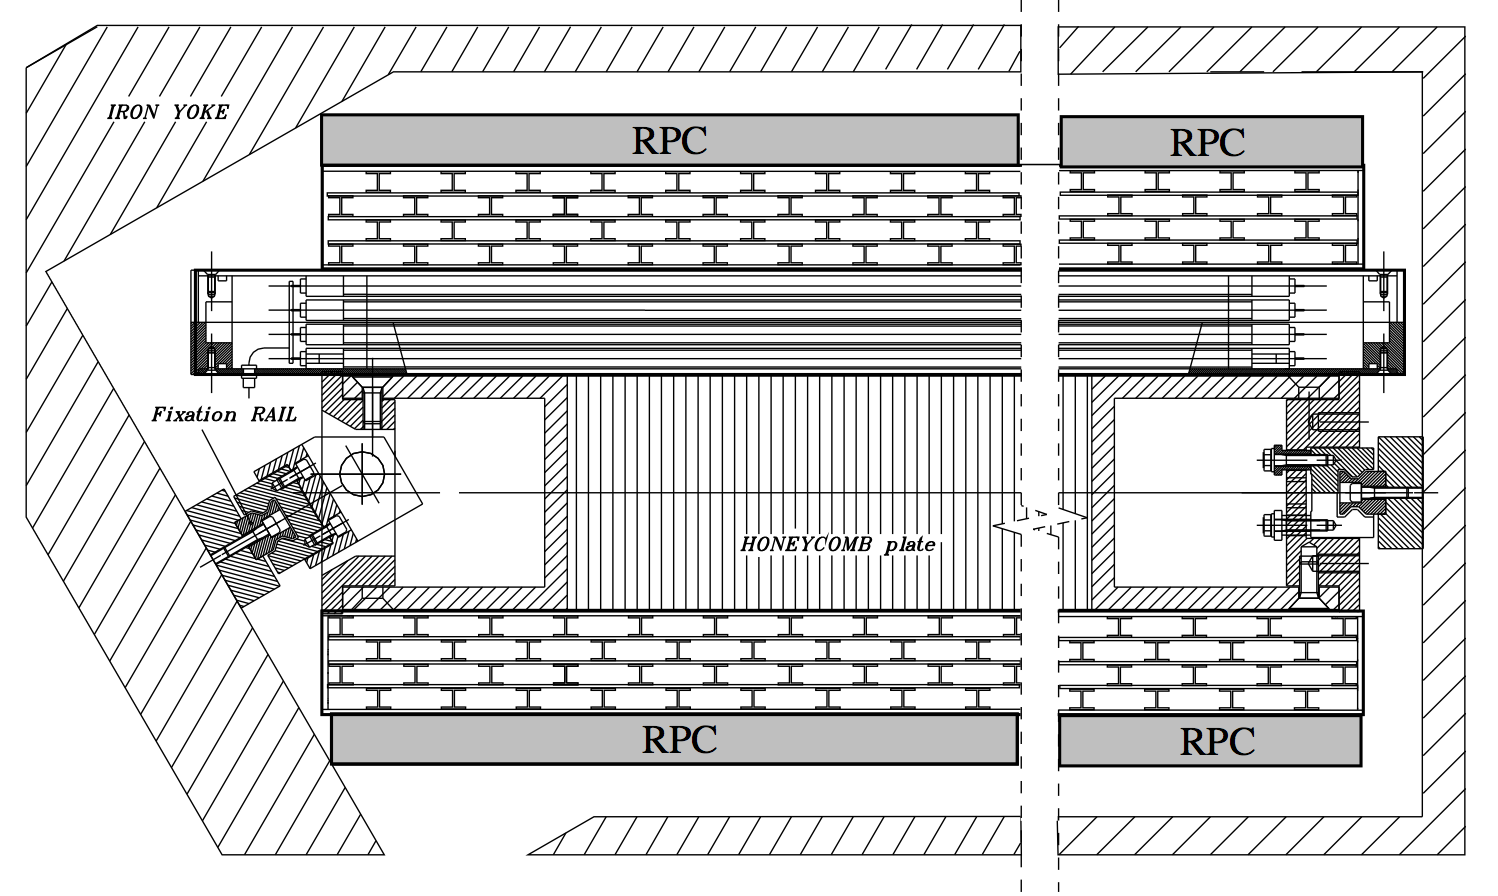
\includegraphics[angle=-0,width=0.8\textwidth]{2_LHC_and_CMS/pics/cms_dt.png}
\caption{Cross-section view of a DT module.
\label{fig:dt_module}
}
\end{center}
\end{figure}


Each SL is made of four stacked layers of drift tubes, staggered by half a cell. This configurations eliminates blind spots and allows for an easy measurement of the muon crossing time by averaging the drift times. Each tube has a rectangular cross-section of $13\times42$ mm\sq ~and is filled with a gas mixture of 85\% Ar and 15\% CO$_2$, leading to a maximum drift time of 380 ns. Each SL has a spatial resolution of about 200 \u m and a time jitter below 5 ns.

\subsubsection*{Cathode Strip Chambers}

The front wheels of the solenoid return yoke are instrumented with multi-wire proportional chambers. Each module has trapezoidal shape and covers either $10\deg$ or $20\deg$ in $\phi$, forming a full disk perpendicular to the beam axis ($r-\phi$ plane). Each of these chambers has the cathode segmented radially in strips (hence the name Cathode Strip Chamber, CSC) of constant $\Delta\phi$ and wires running perpendicular to the strips,  with a wire spacing of 3.2 mm. 

This design allows to cope with the much higher rate with respect to the barrel and with non uniform and non zero magnetic field. 

The CSC detector provides at least three measured space points for muons crossing through its acceptance ($1.2 < |\eta| < 2.4$) and provides a design resolution of approximately 2 mm at trigger level and around 200 \u m after offline reconstruction.

\subsubsection*{Resistive Plate Chambers}

Dual-gap RPC's provide a redundant set of spatial measurements particularly important for trigger purposes, given that their response time is much shorter than 25~ns. The layout chosen by the CMS collaboration consist of six RPC stations in the barrel and three in the endcaps. RPC stations are placed in proximity (before or after) each CSC or DT station. The first two DT stations have two RPC layers on each side of the DT station, providing at least four position measurements, even for low-$p_T$ muons, which might not reach the outer stations. Each chamber is operated in avalanche mode and consist of two gaps sharing a segmented pick-up read-out in between, which allows to operate the chambers at lower voltages (and therefore lower noise) for the same gain. 

\subsection{Trigger}

As previously said, during the years 2010--2012 the LHC operated at bunch crossing period of %delivered an interaction every 
50 ns leading to a 20 MHz frequency, half of the design value.
This frequency is well above the storage capabilities of the most modern technologies, which allow to record a few hundred events per second. The inclusive p-p cross-section is hugely dominated by low-$x$ QCD processes that are of no or little interest for this experiment. 
This leads to the obvious necessity of a fast-logic to isolate events of some interest for the experiment's physics program while rejecting the others. 
The logic to perform this selection, usually referred to as \emph{trigger}, is divided in two stages in case of the CMS experiment: the \emph{level one} (L1) trigger and the \emph{high level trigger} (HLT). 

The L1 trigger decision is based on a coarse reconstruction of the event, performed by custom electronics that is mostly mounted directly on the detector. 
The maximum processing time (called \emph{latency}) is 3.2 \u s. 
During this time the event is stored on the detector electronics in pipelined memories. 
Due to timing constraints only the information provided by the calorimeters and by the muon system is processed. 
For the purpose of the trigger, the calorimeter segmentation is reduced into the so-called \emph{trigger-towers}. 
The calorimeters provide to the trigger logic a set of relevant physics variables like the missing transverse energy ($E_T^{miss}$), the scalar sum of the transverse hadronic activity ($H_T$), the number of jets above different energy thresholds and the locations of towers compatible with a \emph{minimal ionizing particle} (MIP) and information on particle isolation. 
Electron and photon identification is also performed by the trigger by looking at the jet hadronic over electromagnetic energy ratio ($H/E$) plus cluster shape information, the latter being performed with the aid of a look-up table. 
Muon information is mainly provided by DT and CSC subdetectors that are complemented by timing information provided by the RPC for the purpose of determining the correct bunch crossing as well as the removal of ghost-tracks. 
Muon trajectories are first reconstructed coarsely by the detector dedicated electronics and then are sent to a dedicated module which merges the information of different stations and subdetectors, to assess the transverse momentum  and charge. 
%These informations are complemented by those coming from the calorimeters providing isolation values.

The final trigger decision is taken by modules that are located outside the detector volume. These modules exploit FPGA's to achieve fast response while allowing for modification of the algorithms to cope with the evolution the instantaneous luminosity or new physics demands. The maximum output frequency for L1 is 100 kHz.

Once the L1 trigger decision is made the full event is read out from the detector buffers and is sent to the online \emph{Data Quality Monitoring} (DQM) and to the HLT farm, consisting of over a thousand commercial processors working in parallel. During the HLT decision, a simplified version of the CMS offline event reconstruction is performed. Time consuming tasks such as tracking are performed only around the objects that caused the L1 trigger to fire and more complex algorithms like \b-tagging and \t~identification are performed with a simplified version of the code that is used for the final reconstruction. 
The algorithms running at the HLT level %During this trigger stage, decisions are taken on the basis of more complex algorithms and a more refined reconstruction, which allows to 
reduce the event rate to roughly 300Hz, within the storage and processing capabilities of the CERN facilities. Being completely software-based, the HLT is far more flexible and fast evolving than the L1 trigger, which allowed it to adjust well to the rapidly evolving machine conditions during the 2010--2012 data-taking periods. The performance achieved during data-taking have been beyond the most optimistic forecasts made at the start-up.
%allowing to cope with the fast changing machine conditions during 2010 and 2011 runs and achieving a level of refinement beyond the most optimistic forecasts made at the start-up.

Once one event gets accepted by the HLT, it is transferred to the CERN computing center for storage and reconstruction.

\section{Data storage and processing}

Event information recorded by the detector is stored in \emph{RAW} data format, which contains all the digitalized output of the single subdetectors plus L1 and HLT information. In order to be useful for physics analysis, the trajectory and the type of all particles produced in the proton-proton collision must be inferred based on the digitized hits stored in the RAW event content. This process is usually called event reconstruction and is the topic of the following chapter. The CMS detector produces about 15 TB of data for each day of operation.

The reconstruction of collected and simulated data is too CPU and storage demanding to be delegated to a single facility. In order to evenly spread the computing load, a new computing model has been created, involving different computing facilities in various parts of the world. The \emph{world wide computing grid} \cite{Malecki:2005gn} allows for fast data transfer plus de-localized reconstruction and analysis of data throughout the world, satisfying the huge computing demands that the LHC experiments need in order to operate successfully. 

In some sense the grid can be seen as an extension of the batch queue system where the user submits jobs to a single machine, whereas, in this case, he submits them to clusters of machines, that then take care of submitting those jobs in their peculiar batch queue implementation. Computing facilities are organized in a hierarchical structure called tiers, starting from the facility that receives the data from the detector, called Tier0, scaling to smaller and smaller facilities up to Tier3's which provide limited computing and storage for local groups. In this architechture secure access to the resources is ensured by a system of certificates spawning children proxies of limited lifetime.

%displayed
%presented
%illustrated